\documentclass[12pt,letterpaper]{article}
\usepackage{graphicx,textcomp}
\usepackage{natbib}
\usepackage{setspace}
\usepackage{fullpage}
\usepackage{color}
\usepackage[reqno]{amsmath}
\usepackage{amsthm}
\usepackage{fancyvrb}
\usepackage{amssymb,enumerate}
\usepackage[all]{xy}
\usepackage{endnotes}
\usepackage{lscape}
\newtheorem{com}{Comment}
\usepackage{float}
\usepackage{hyperref}
\newtheorem{lem} {Lemma}
\newtheorem{prop}{Proposition}
\newtheorem{thm}{Theorem}
\newtheorem{defn}{Definition}
\newtheorem{cor}{Corollary}
\newtheorem{obs}{Observation}
\usepackage[compact]{titlesec}
\usepackage{dcolumn}
\usepackage{tikz}
\usetikzlibrary{arrows}
\usepackage{multirow}
\usepackage{xcolor}
\newcolumntype{.}{D{.}{.}{-1}}
\newcolumntype{d}[1]{D{.}{.}{#1}}
\definecolor{light-gray}{gray}{0.65}
\usepackage{url}
\usepackage{listings}
\usepackage{color}

\definecolor{codegreen}{rgb}{0,0.6,0}
\definecolor{codegray}{rgb}{0.5,0.5,0.5}
\definecolor{codepurple}{rgb}{0.58,0,0.82}
\definecolor{backcolour}{rgb}{0.95,0.95,0.92}

\lstdefinestyle{mystyle}{
	backgroundcolor=\color{backcolour},   
	commentstyle=\color{codegreen},
	keywordstyle=\color{magenta},
	numberstyle=\tiny\color{codegray},
	stringstyle=\color{codepurple},
	basicstyle=\footnotesize,
	breakatwhitespace=false,         
	breaklines=true,                 
	captionpos=b,                    
	keepspaces=true,                 
	numbers=left,                    
	numbersep=5pt,                  
	showspaces=false,                
	showstringspaces=false,
	showtabs=false,                  
	tabsize=2
}
\lstset{style=mystyle}
\newcommand{\Sref}[1]{Section~\ref{#1}}
\newtheorem{hyp}{Hypothesis}

\title{Problem Set 3}
\date{Due: November 11, 2024}
\author{Applied Stats/Quant Methods 1}


\begin{document}
	\maketitle
	\vspace{-2em} 
	\noindent \textbf{Name: Eimhin ONeill} \\
	\noindent \textbf{Student Number: 20332107} \\
	
	\section*{Instructions}
	\begin{itemize}
		\item Please show your work! You may lose points by simply writing in the answer. If the problem requires you to execute commands in \texttt{R}, please include the code you used to get your answers. Please also include the \texttt{.R} file that contains your code. If you are not sure if work needs to be shown for a particular problem, please ask.
	\item Your homework should be submitted electronically on GitHub.
	\item This problem set is due before 23:59 on Monday November 11, 2024. No late assignments will be accepted.

	\end{itemize}

		\vspace{.25cm}
	
\noindent In this problem set, you will run several regressions and create an add variable plot (see the lecture slides) in \texttt{R} using the \texttt{incumbents\_subset.csv} dataset. Include all of your code.

	\vspace{.5cm}
\section*{Question 1}
\vspace{.25cm}
\noindent We are interested in knowing how the difference in campaign spending between incumbent and challenger affects the incumbent's vote share. 
	\begin{enumerate}
		\item Run a regression where the outcome variable is \texttt{voteshare} and the explanatory variable is \texttt{difflog}.	\vspace{1cm}
		
		\lstinputlisting[language=R, firstline=52, lastline=52]{/Users/eimhi/Documents/GitHub/StatsI_Fall2024/problemSets/PS03/MY WORK/PS03.R}  
		
		\vspace{2cm}
		
		\item Make a scatterplot of the two variables and add the regression line.
		\vspace{1cm}
		
		\lstinputlisting[language=R, firstline=55, lastline=61]{/Users/eimhi/Documents/GitHub/StatsI_Fall2024/problemSets/PS03/MY WORK/PS03.R}  
		
		\vspace{1cm}
		
		 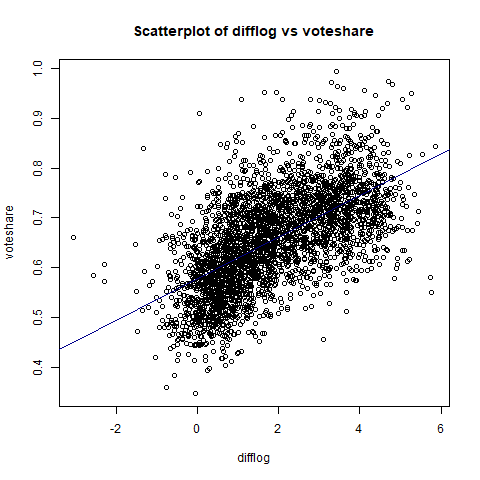
\includegraphics[width=0.8\textwidth]{/Users/eimhi/Documents/GitHub/StatsI_Fall2024/problemSets/PS03/MY WORK/vs_difflog_plot.png}
		
		\vspace{1cm}
		
		\item Save the residuals of the model in a separate object.
		\vspace{1cm}
		
		\lstinputlisting[language=R, firstline=64, lastline=65]{/Users/eimhi/Documents/GitHub/StatsI_Fall2024/problemSets/PS03/MY WORK/PS03.R}  
		
		\vspace{1cm}
		
		\item Write the prediction equation.
			\vspace{1cm}
		
		\lstinputlisting[language=R, firstline=68, lastline=78]{/Users/eimhi/Documents/GitHub/StatsI_Fall2024/problemSets/PS03/MY WORK/PS03.R}  
		
		\vspace{1cm}
		
		
	\end{enumerate}
	
\newpage

\section*{Question 2}
\noindent We are interested in knowing how the difference between incumbent and challenger's spending and the vote share of the presidential candidate of the incumbent's party are related.	\vspace{.25cm}
	\begin{enumerate}
		\item Run a regression where the outcome variable is \texttt{presvote} and the explanatory variable is \texttt{difflog}.	\vspace{1cm}
		
		\lstinputlisting[language=R, firstline=90, lastline=90]{/Users/eimhi/Documents/GitHub/StatsI_Fall2024/problemSets/PS03/MY WORK/PS03.R}  
		
		\vspace{1cm}
		
		\item Make a scatterplot of the two variables and add the regression line. 	
		\vspace{1cm}
		
		\lstinputlisting[language=R, firstline=52, lastline=52]{/Users/eimhi/Documents/GitHub/StatsI_Fall2024/problemSets/PS03/MY WORK/PS03.R}  
	
		\vspace{1cm}
		
		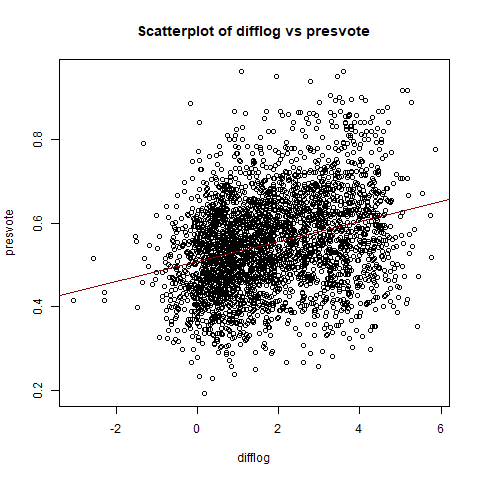
\includegraphics[width=0.8\textwidth]{/Users/eimhi/Documents/GitHub/StatsI_Fall2024/problemSets/PS03/MY WORK/pv_difflog_plot.png}
		
		\vspace{1cm}
		
		\item Save the residuals of the model in a separate object.	
			\vspace{1cm}
		
		\lstinputlisting[language=R, firstline=102, lastline=103]{/Users/eimhi/Documents/GitHub/StatsI_Fall2024/problemSets/PS03/MY WORK/PS03.R}  
		
		\vspace{1cm}
		
		\item Write the prediction equation.
			\vspace{1cm}
		
		\lstinputlisting[language=R, firstline=106, lastline=113]{/Users/eimhi/Documents/GitHub/StatsI_Fall2024/problemSets/PS03/MY WORK/PS03.R}  
		
		\vspace{1cm}
	\end{enumerate}
	
	\newpage	
\section*{Question 3}

\noindent We are interested in knowing how the vote share of the presidential candidate of the incumbent's party is associated with the incumbent's electoral success.
	\vspace{.25cm}
	\begin{enumerate}
		\item Run a regression where the outcome variable is \texttt{voteshare} and the explanatory variable is \texttt{presvote}.
			\vspace{1cm}
			
			\lstinputlisting[language=R, firstline=129, lastline=129]{/Users/eimhi/Documents/GitHub/StatsI_Fall2024/problemSets/PS03/MY WORK/PS03.R}  
			
			\vspace{1cm}
			
			
		\item Make a scatterplot of the two variables and add the regression line. 
		\vspace{1cm}
		
		\lstinputlisting[language=R, firstline=132, lastline=138]{/Users/eimhi/Documents/GitHub/StatsI_Fall2024/problemSets/PS03/MY WORK/PS03.R}  
		
		\vspace{1cm}
		
		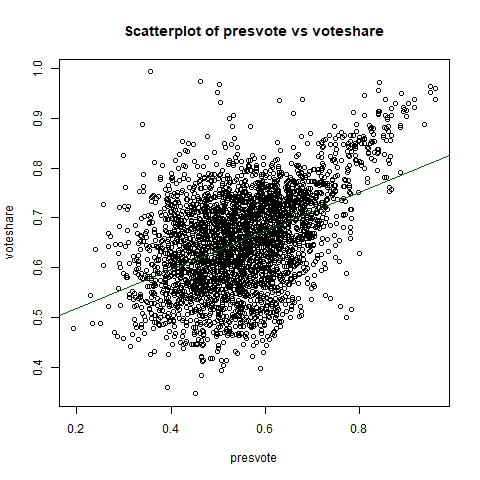
\includegraphics[width=0.8\textwidth]{/Users/eimhi/Documents/GitHub/StatsI_Fall2024/problemSets/PS03/MY WORK/vs_pv_plot.png}
		
		\vspace{1cm}
		
		\item Write the prediction equation.
		\vspace{1cm}
		
		\lstinputlisting[language=R, firstline=145, lastline=154]{/Users/eimhi/Documents/GitHub/StatsI_Fall2024/problemSets/PS03/MY WORK/PS03.R}  
		
		\vspace{1cm}
	\end{enumerate}
	

\newpage	
\section*{Question 4}
\noindent The residuals from part (a) tell us how much of the variation in \texttt{voteshare} is $not$ explained by the difference in spending between incumbent and challenger. The residuals in part (b) tell us how much of the variation in \texttt{presvote} is $not$ explained by the difference in spending between incumbent and challenger in the district.
	\begin{enumerate}
		\item Run a regression where the outcome variable is the residuals from Question 1 and the explanatory variable is the residuals from Question 2.	
		\vspace{1cm}
		
		\lstinputlisting[language=R, firstline=171, lastline=171]{/Users/eimhi/Documents/GitHub/StatsI_Fall2024/problemSets/PS03/MY WORK/PS03.R}  
		
		\vspace{1cm}
		
		\item Make a scatterplot of the two residuals and add the regression line.
		\vspace{1cm}
		
		\lstinputlisting[language=R, firstline=174, lastline=180]{/Users/eimhi/Documents/GitHub/StatsI_Fall2024/problemSets/PS03/MY WORK/PS03.R}  
		\vspace{1cm}
		
		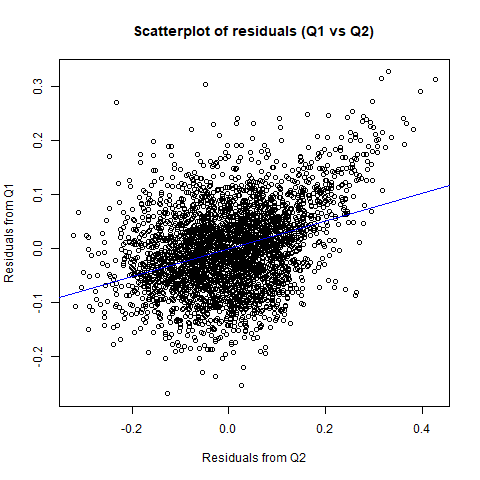
\includegraphics[width=0.8\textwidth]{/Users/eimhi/Documents/GitHub/StatsI_Fall2024/problemSets/PS03/MY WORK/resid_plot.png}
		
		\vspace{1cm}
		
		
		\item Write the prediction equation.
		\vspace{1cm}
		
		\lstinputlisting[language=R, firstline=183, lastline=193]{/Users/eimhi/Documents/GitHub/StatsI_Fall2024/problemSets/PS03/MY WORK/PS03.R}  
		
		\vspace{1cm}
	\end{enumerate}
	
	\newpage	

\section*{Question 5}
\noindent What if the incumbent's vote share is affected by both the president's popularity and the difference in spending between incumbent and challenger? 
	\begin{enumerate}
		\item Run a regression where the outcome variable is the incumbent's \texttt{voteshare} and the explanatory variables are \texttt{difflog} and \texttt{presvote}.	\vspace{1cm}
		
		\lstinputlisting[language=R, firstline=204, lastline=204]{/Users/eimhi/Documents/GitHub/StatsI_Fall2024/problemSets/PS03/MY WORK/PS03.R}  
		
		\vspace{1cm}
		
		
		\item Write the prediction equation.	\vspace{1cm}
		
		\lstinputlisting[language=R, firstline=207, lastline=222]{/Users/eimhi/Documents/GitHub/StatsI_Fall2024/problemSets/PS03/MY WORK/PS03.R}  
		
		\vspace{1cm}
		
		
		\item What is it in this output that is identical to the output in Question 4? Why do you think this is the case?
		
		\vspace{1cm}
		
		The slope for presvote (0.2569) here is identical to the slope from Question 4’s regression of Q.1's residuals on Q.2's residuals (0.2569). This happens because both isolate the relationship between presvote and voteshare, and control for difflog. In this question, it's isolated within the context of a multiple regression with both predictors, but for Q4, it's isolated by analysing the residuals, or more simply, the variation not explained by difflog. 
		
		 \vspace{1cm}
		 
		 Overall, this confirms presvote's indepndent effect on voteshare, irrespective of difflog.
		
		
	\end{enumerate}




\end{document}
